% Options for packages loaded elsewhere
\PassOptionsToPackage{unicode}{hyperref}
\PassOptionsToPackage{hyphens}{url}
%
\documentclass[
  12pt]{article}
\usepackage{amsmath,amssymb}
\usepackage{iftex}
\ifPDFTeX
  \usepackage[T1]{fontenc}
  \usepackage[utf8]{inputenc}
  \usepackage{textcomp} % provide euro and other symbols
\else % if luatex or xetex
  \usepackage{unicode-math} % this also loads fontspec
  \defaultfontfeatures{Scale=MatchLowercase}
  \defaultfontfeatures[\rmfamily]{Ligatures=TeX,Scale=1}
\fi
\usepackage{lmodern}
\ifPDFTeX\else
  % xetex/luatex font selection
\fi
% Use upquote if available, for straight quotes in verbatim environments
\IfFileExists{upquote.sty}{\usepackage{upquote}}{}
\IfFileExists{microtype.sty}{% use microtype if available
  \usepackage[]{microtype}
  \UseMicrotypeSet[protrusion]{basicmath} % disable protrusion for tt fonts
}{}
\makeatletter
\@ifundefined{KOMAClassName}{% if non-KOMA class
  \IfFileExists{parskip.sty}{%
    \usepackage{parskip}
  }{% else
    \setlength{\parindent}{0pt}
    \setlength{\parskip}{6pt plus 2pt minus 1pt}}
}{% if KOMA class
  \KOMAoptions{parskip=half}}
\makeatother
\usepackage{xcolor}
\usepackage{graphicx}
\makeatletter
\def\maxwidth{\ifdim\Gin@nat@width>\linewidth\linewidth\else\Gin@nat@width\fi}
\def\maxheight{\ifdim\Gin@nat@height>\textheight\textheight\else\Gin@nat@height\fi}
\makeatother
% Scale images if necessary, so that they will not overflow the page
% margins by default, and it is still possible to overwrite the defaults
% using explicit options in \includegraphics[width, height, ...]{}
\setkeys{Gin}{width=\maxwidth,height=\maxheight,keepaspectratio}
% Set default figure placement to htbp
\makeatletter
\def\fps@figure{htbp}
\makeatother
\setlength{\emergencystretch}{3em} % prevent overfull lines
\providecommand{\tightlist}{%
  \setlength{\itemsep}{0pt}\setlength{\parskip}{0pt}}
\setcounter{secnumdepth}{-\maxdimen} % remove section numbering
\newlength{\cslhangindent}
\setlength{\cslhangindent}{1.5em}
\newlength{\csllabelwidth}
\setlength{\csllabelwidth}{3em}
\newlength{\cslentryspacingunit} % times entry-spacing
\setlength{\cslentryspacingunit}{\parskip}
\newenvironment{CSLReferences}[2] % #1 hanging-ident, #2 entry spacing
 {% don't indent paragraphs
  \setlength{\parindent}{0pt}
  % turn on hanging indent if param 1 is 1
  \ifodd #1
  \let\oldpar\par
  \def\par{\hangindent=\cslhangindent\oldpar}
  \fi
  % set entry spacing
  \setlength{\parskip}{#2\cslentryspacingunit}
 }%
 {}
\usepackage{calc}
\newcommand{\CSLBlock}[1]{#1\hfill\break}
\newcommand{\CSLLeftMargin}[1]{\parbox[t]{\csllabelwidth}{#1}}
\newcommand{\CSLRightInline}[1]{\parbox[t]{\linewidth - \csllabelwidth}{#1}\break}
\newcommand{\CSLIndent}[1]{\hspace{\cslhangindent}#1}
\ifLuaTeX
\usepackage[bidi=basic]{babel}
\else
\usepackage[bidi=default]{babel}
\fi
\babelprovide[main,import]{spanish}
% get rid of language-specific shorthands (see #6817):
\let\LanguageShortHands\languageshorthands
\def\languageshorthands#1{}
\usepackage{makeidx}
\makeindex
\usepackage{graphicx}
\usepackage{tikz}
\usepackage{atbegshi}

\AtBeginDocument{
    \AtBeginShipoutNext{
        \AtBeginShipoutUpperLeft{
            \put(\dimexpr\paperwidth/2-\textwidth/2\relax, -650){
                \makebox[\textwidth]{
                    
\includegraphics[width=0.45\textwidth]{cure_udelar.png}  % Adjust width as needed
                    \hfill
                    
\includegraphics[width=0.405\textwidth]{logoMEDIA.jpeg} % Make it 90% smaller
                }
            }
        }
    }
}
\ifLuaTeX
  \usepackage{selnolig}  % disable illegal ligatures
\fi
\IfFileExists{bookmark.sty}{\usepackage{bookmark}}{\usepackage{hyperref}}
\IfFileExists{xurl.sty}{\usepackage{xurl}}{} % add URL line breaks if available
\urlstyle{same}
\hypersetup{
  pdftitle={Entrega: Curso De Datos Extremales},
  pdfauthor={Laura Montaldo, CI: 3.512.962-7},
  pdflang={es},
  hidelinks,
  pdfcreator={LaTeX via pandoc}}

\title{Entrega: Curso De Datos Extremales}
\author{Laura Montaldo, CI: 3.512.962-7}
\date{2024-02-08}

\begin{document}
\maketitle

\newpage

\thispagestyle{empty}

\maketitle

\newpage

\tableofcontents

\newpage

\hypertarget{resumen}{%
\section{Resumen}\label{resumen}}

Your abstract goes here.

\newpage

\hypertarget{motivaciuxf3n-y-objetivo-del-estudio}{%
\section{Motivación y objetivo del
estudio}\label{motivaciuxf3n-y-objetivo-del-estudio}}

Los índices de \(S\&P\) son una familia de índices de renta
variable\footnote{En inglés se llaman equity indices} diseñados para
medir el rendimiento del mercado de acciones en Estados Unidos que
cotizan en bolsas estadounidenses. Ésta familia de índices está
compuesta por una amplia variedad de índices basados en tamaño, sector y
estilo. Los índices están ponderados por el criterio
\textit{float-adjusted market capitalization} (FMC). Además, se disponen
de índices ponderados de manera equitativa y con límite de
capitalización de mercado, como es el caso del \(S\&P\:500\). Este este
sentido, el \(S\&P 500\) entraría en el conjunto de índices ponderados
por capitalización bursátil ajustada a la flotación (ver
\href{http://www.overleaf.com}{\textcolor{blue}{$S\&P$ Dow Jones Indices}}).
El mismo mide el rendimiento del segmento de gran capitalización del
mercado estadounidense. Es considerado como un indicador representativo
del mercado de renta variable de los Estados Unidos, y está compuesto
por 500 empresas constituyentes.

Se busca crear un indicador de una posible crisis bursátil. Como
variable de referencia de toma la relación de precios al cierre de ayer
sobre la de hoy

\begin{equation}
Indicador_t=\frac{Precio_{t-1}}{Precio_t},\quad\text{para}\; t=1,...,T \label{eq:ind}
\end{equation} \vspace{0.5cm}

Interpretación del Indicador:

\begin{itemize}
\item Si el $Indicador_t$    $\leq$ 1, el precio de cierre de hoy es mayor o igual que el de ayer, lo cual podría ser considerado una señal positiva.
\item Si el $Indicador_t$ > 1, el precio de cierre de hoy es menor que el de ayer, lo cual podría considerarse una señal de alerta.
\end{itemize}

\vspace{1cm}

En las siguiente figura @ref(fig:plot1) se muestra la evolución
histórica desde la fecha 03/01/1928 hasta 08/12/2023 del precio al
cierre del día del indicar S\&P 500.

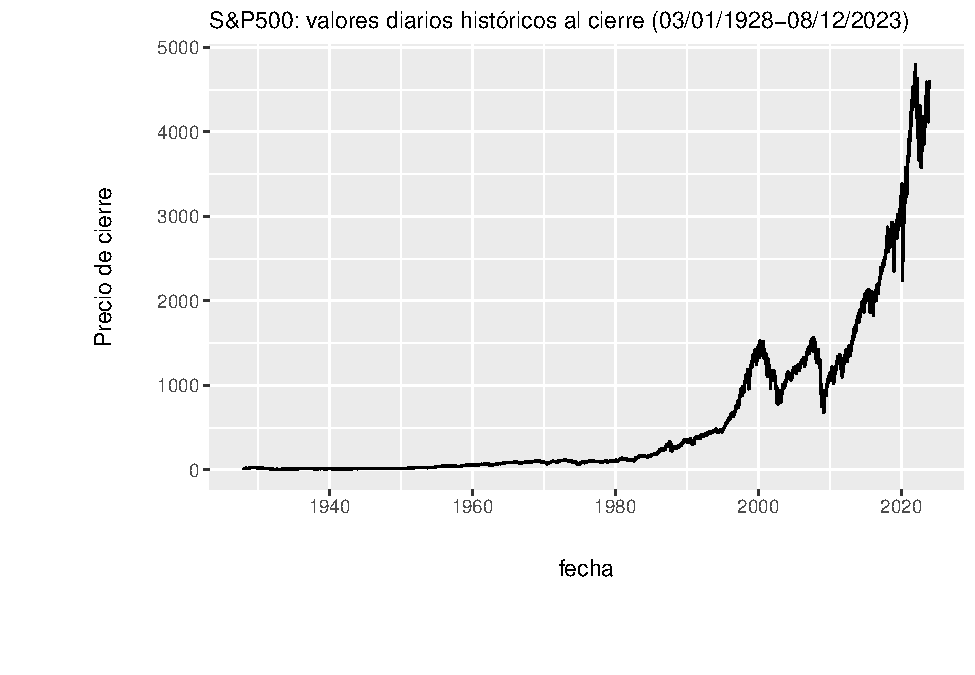
\includegraphics{extremales_files/figure-latex/plot1-1.pdf}

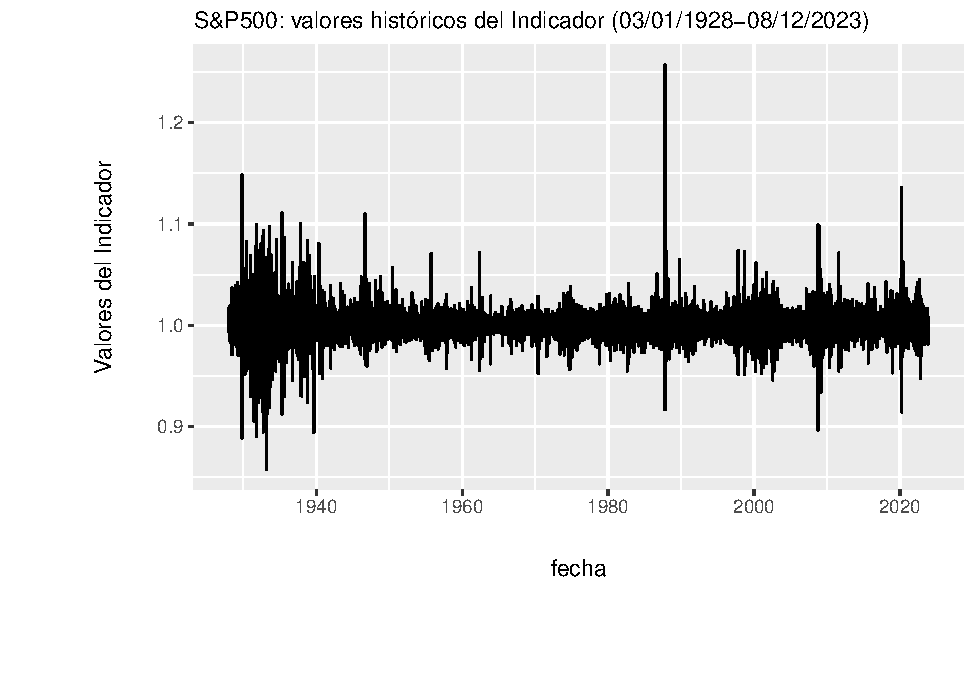
\includegraphics{extremales_files/figure-latex/plot2-1.pdf} \newpage

\hypertarget{marco-teuxf3rico}{%
\section{Marco Teórico}\label{marco-teuxf3rico}}

\hypertarget{teoruxeda-asintuxf3tica-cluxe1sica-y-las-distribuciones-extremales-y-sus-dominios-de-atracciuxf3n}{%
\subsection{Teoría asintótica clásica y las distribuciones extremales y
sus dominios de
atracción}\label{teoruxeda-asintuxf3tica-cluxe1sica-y-las-distribuciones-extremales-y-sus-dominios-de-atracciuxf3n}}

Siguiendo Gonzalo y Segura (2024) se dice que tenemos datos extremos
cuando cada dato corresponde al máximo o mínimo de varios registros. Son
un caso particular de evento raro o gran desviación respecto a la media.

Asumiremos que nuestros datos son \(iid\) (independientes e
idénticamente distribuidos, son dos suposiciones juntas). Esta doble
suposición suele no ser realista en aplicaciones concretas (ninguna de
sus dos componentes, incluso) pero para comenzar a entender la teoría
clásica, la utilizaremos por un tiempo.

Si tenemos datos \(X_1,...,X_n\) \(iid\) con distribución \(F\),
entonces \(X_n^* = max (X_1,...,X_n)\) tiene distribución \(F_n^*\) dada
por \(F_n^* (t)= F(t)_n\). Si conocemos la distribución \(F\)
conoceríamos la distribución \(F_n^*\) , pero en algunos casos la
lectura que queda registrada es la del dato máximo y no la de cada
observación que dio lugar al mismo, por lo que a veces ni siquiera es
viable estimar \(F\). Pero aún en los casos en que \(F\) es conocida o
estimable, si \(n\) es grande, la fórmula de \(F_n^*\) puede resultar
prácticamente inmanejable. En una línea de trabajo similar a la que
aporta el Teorema Central del Límite en la estadística de valores
medios, un teorema nos va a permitir aproximar \(F_n^*\) por
distribuciones más sencillas. Este es el Teorema de
Fischer-Tippet-Gnedenko (FTG, para abreviar) que presentaremos en breve.

Como \(X_1,...,X_n\) iid, definimos \(Y_i = -X_i\) para todo valor de
\(i\), entonces \(Y_1,...,Y_n\) iid y además
\(min(X_1,...,X_n) = - max(Y_1,...,Y_n)\) la teoría asintótica de los
mínimos de datos iid se reduce a la de los máximos, razón por la que nos
concentramos aquí en estudiar el comportamiento asintótico de los
máximos exclusivamente.

\newpage

\hypertarget{las-distribuciones-extremales}{%
\subsection{Las distribuciones
extremales}\label{las-distribuciones-extremales}}

Las distribuciones extremales son tres: la distribución de Gumbel; la
distribución de Weibull; la distribución de Fréchet.

\hypertarget{distribuciuxf3n-de-gumbel}{%
\subsubsection{Distribución de Gumbel}\label{distribuciuxf3n-de-gumbel}}

Se dice que una variable tiene distribución de Gumbel si su distribución
es:

\[ \Lambda(x) = exp\{-e^{-x}\} \quad\text{para todo}\; x \;\text{real} \]

\hypertarget{distribuciuxf3n-de-weibull}{%
\subsubsection{Distribución de
Weibull}\label{distribuciuxf3n-de-weibull}}

Se dice que una variable tiene distribución de Weibull de orden
\(\alpha>0\) si su distribución es:

\[\Psi_{\alpha}(x)=\begin{cases}
exp{-(-x)^{\alpha}} & si\;x<0\\
1 & \text{en otro caso}
\end{cases}\]

\hypertarget{distribuciuxf3n-de-fruxe9chet}{%
\subsubsection{Distribución de
Fréchet}\label{distribuciuxf3n-de-fruxe9chet}}

Se dice que una variable tiene distribución de Fréchet de orden
\(\alpha>0\) si su distribución es:

\[
\Phi_{\alpha}(x)=\begin{cases}
exp\{-x^{-\alpha}\} & si\;x>0\\
0 & \text{en otro caso}
\end{cases}
\] \newpage

\hypertarget{teorema-1-relaciones-entre-las-versiones-standard-de-las-distribuciones-extremales}{%
\subsubsection{Teorema 1: Relaciones entre las versiones standard de las
distribuciones
extremales}\label{teorema-1-relaciones-entre-las-versiones-standard-de-las-distribuciones-extremales}}

\(X\) tiene distribución \(\Phi_{\alpha}(x)\) si y sólo si \((-1/X)\)
tiene distribución \(\Psi_{\alpha}(x)\) si y sólo si \(log(X^{\alpha})\)
tiene distribución \(\Lambda\).

\hypertarget{teorema-2-algunos-datos-de-las-distribuciones-extremales}{%
\subsubsection{Teorema 2: Algunos datos de las distribuciones
extremales}\label{teorema-2-algunos-datos-de-las-distribuciones-extremales}}

\hypertarget{parte-1}{%
\paragraph{Parte 1}\label{parte-1}}

Si \(X\) tiene distribución \(\Lambda^{(\mu,\beta)}\) entonces tiene:

\begin{itemize}
  \item[a)] Valor esperado: $E(X) = \mu + \beta\gamma$, donde $\gamma$ es la constante de Euler-Mascheroni, cuyo valor aproximado es $0.5772156649$.
  \item[b)] Moda: $\mu$
  \item[c)] Mediana: $\mu - \beta \log(\log 2) \approx \mu - 0.36651 \beta$.
  \item[d)] Desviación estándar: $\beta \pi \sqrt{6} \approx 1.2825 \beta$.
  \item[e)] Si $X^+ = \max(X,0)$, entonces $E(X+k)$ es finito para todo valor de $k$ natural.
  \item[f)] Para simular computacionalmente $X$, se puede tomar $U$ uniforme en $(0,1)$ y hacer $X = \mu - \beta \log(-\log U)$.
\end{itemize}

\hypertarget{parte-2}{%
\paragraph{Parte 2}\label{parte-2}}

Si \(X\) tiene distribución \(\Psi_{\alpha}^{(\mu,\beta)}\) entonces
tiene:

\begin{itemize}
  \item[a)] Valor esperado: $E(X) = \mu + \beta\Gamma(1+1/\alpha)$.
  \item[b)] Moda: $\mu$ si $\alpha\leq 1$ y $\mu-\beta\{(\alpha-1)/\alpha\}^{(1/\alpha)}$ si $\alpha>1$.
  \item[c)] Mediana: $\mu - \beta \log(2)^{(1/\alpha)}$.
  \item[d)] Desviación estándar: $\beta\{\Gamma(1+2/\alpha)-\Gamma(1+1/\alpha)^2\}^{1/2}$.
\end{itemize}

\hypertarget{parte-2-1}{%
\paragraph{Parte 2}\label{parte-2-1}}

Si \(X\) tiene una distribución \(\Phi_{\alpha}^{(\mu, \beta)}\)
entonces se tiene:

\begin{itemize}
  \item[a)] Valor esperado: $E(X) = \mu + \beta\Gamma(1-1/\alpha)$ si $\alpha > 1$, $\infty$ en caso contrario.
  \item[b)] Moda: $\mu + \beta\Gamma(1-1/\alpha)$ si $\alpha>1$.
  \item[c)] Mediana: $\mu + \beta \log(2)^{(-1/\alpha)}$.
  \item[d)] Desviación estándar: $\beta|\Gamma(1-2/\alpha)-\Gamma(1-1/\alpha)^2|$ si $\alpha>2$, $\infty$ si $1<\alpha \leq 2$.
\end{itemize}

\newpage

\hypertarget{teorema-3-fischer-tippet-gnedenko-ftg}{%
\subsubsection{Teorema 3: Fischer-Tippet-Gnedenko
(FTG)}\label{teorema-3-fischer-tippet-gnedenko-ftg}}

Si \(X_1,...,X_n\quad iid\) con distribución \(F\) ``continua'',
llamamos \(F_n^*\) a la distribución de \(max(X_1,...,X_n)\) y \(n\) es
grande, entonces existen \(\mu\) real y \(\beta>0\) tales que alguna de
las siguientes tres afirmaciones es correcta:

\begin{itemize}
  \item[1)] $F_n^*$ se puede apromixar por la distribución de $\mu+\beta Y$ con $Y$ variable con distribución $\Lambda$.
  \item[2)] Existe $\alpha>0$ tal que $F_n^*$ se puede aproximar por la distribución de $\mu+\beta Y$ con $Y$ variable con distribución $\Phi_{\alpha}$. 
  \item[3)] Existe $\alpha>0$ tal que $F_n^*$ se puede aproximar por la distribución de $\mu+\beta Y$ con $Y$ variable con distribución $\Phi_{\alpha}$.
\end{itemize}

Lo anterior equivale a decir que la distribución del máximo de datos
``continuos'' e \(iid\), si \(n\) es grande, puede aproximarse por una
Gumbel, una Fréchet o una Weibull. Una aproximación será válida
dependiendo de la distribución de \(F\). En este sentido, cuando \(F\)
sea normal entonces \(F_n^*\) se puede aproximar como una Gumbel. Cuando
\(F\) sea uniforme, se puede aproximar \(F_n^*\) como una Weibull y
cuando \(F\) sea Cauchy entonces \(F_n^*\) se puede aproximar por una
Fréchet.

\newpage

\hypertarget{referencias-bibliogruxe1ficas}{%
\section{Referencias
bibliográficas}\label{referencias-bibliogruxe1ficas}}

\vspace{1cm}
\setlength{\parindent}{-0.2in}
\setlength{\leftskip}{0.2in}

\hypertarget{refs}{}
\begin{CSLReferences}{1}{0}
\leavevmode\vadjust pre{\hypertarget{ref-notas_curso}{}}%
Gonzalo, P., Segura, A., 2024. Notas del curso.

\end{CSLReferences}

\end{document}
